\section{Introduction}

\subsection{Adaptive Mutations}

Biologists have long wondered the extent to which evolution occurs due
to nearly neutral and slighly deleterious mutations, or adaptive
mutations, or more complex situations involving these types of
mutations as well as their epistatic interactions (cite the work of
Kimura etc.).

The occurence of beneficial mutations and how they affect adaptation
is currently an area of active interest in evolutionary biology
\citep{Chou2011, Weinreich2006}. Although much focus in the past
has been placed on deleterious mutations because of their prevalence
in nature and disease, it is ultimately beneficial mutations that
are responsible for adaptive evolution.
 
\subsection{Adaptive Mutations and Epistasis}



\subsection{The Need for a New Modeling Framework}
Clearly, using FBA with the growth objective alone is not enough--we
only ever get the optimum for our fitness objective.  A way to
circumvent this issue is to associate a feature of the system
(e.g. flux into biomass) as the fitness while optimizing some other
objective. This latter mechanism is not generally used as most models
tend to be rather under-constrained as is. However, as we've seen, the
FALCON method \hl{cite} and other fitting methods like MoMA provide a
way to use high-throughput data to introduce many additional
constraints to the system.

Having a systems tool that can work with models of particular organisms
will not only add another tool in the computational evolution and
population genetics arsenal, but also in applied fields such as
evolutionary engineering of microbial engineering, and understanding
which gene mutant combinations which may be most advantageous for
a cancer cell population.

\section{Results}

\subsection{Weighted MoMA-FBA Objectives}

Minimization of metabolic adjustment (MoMA), along with Flux Balance
Analysis (FBA), has proven successful in simulating growth rates and
predicting in silico fluxes. Here we discuss a weighted objective
approach that combines both objectives. \hl{Insert some math background
from original \LaTeX~report.} 

The difference in smoothness between weighted quadratic MoMA and linear
MoMA can be illustrated by considering the growth rate to be a
function of the weight placed on the biomass objective (\Fig~\ref{fig:Fitness_LM_QP}).  An
advantage of quadratic MoMA is that it simulates a continuous range of
fitnesses, potentially matching any required fitness level exactly.
However, this is not necessarily always biologically relevant;
discrete mutations may give a discrete jump in fitness. Weighted
linear MoMA models these discrete transitions in flux state, and often
this is reflected in discrete jumps in fitness, as seen above.

\begin{figure}
\centering
  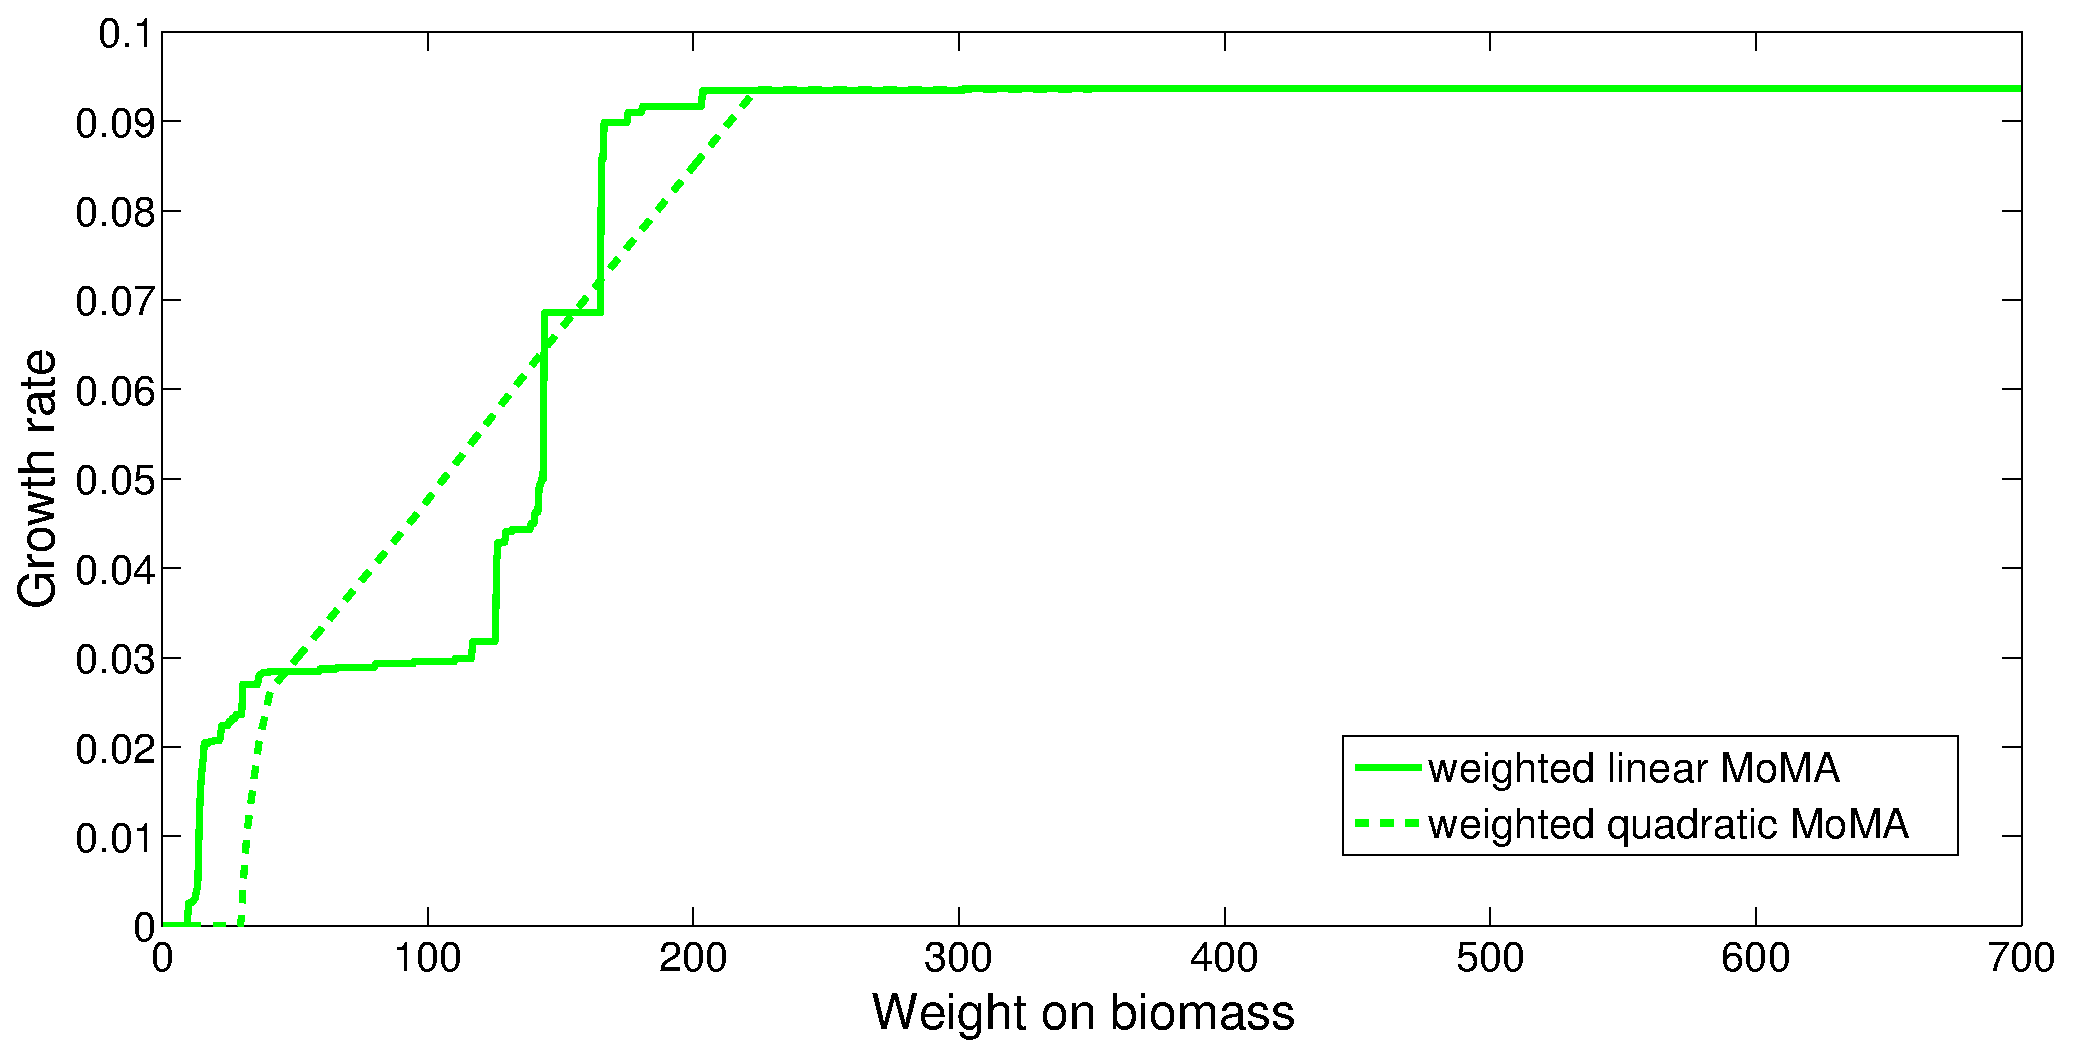
\includegraphics[width=\textwidth]{Fitness_LM_QP}
  \caption{\hl{it is empty}}
  \label{fig:Fitness_LM_QP}
\end{figure}

In the above figure, the difference in fitness between weighted
quadratic MoMA and linear MoMA can be seen. An advantage of quadratic
MoMA is that it simulates a continuous range of fitnesses, potentially
matching any required fitness level exactly.  However, this is not
necessarily always biologically relevant; in reality, discrete mutations may give
a discrete jump in fitness. Weighted linear MoMA models these discrete
transitions in flux state, and often this is reflected in discrete
jumps in fitness, as seen above.

\subsubsection{Weighted MoMA predicts expression states}

Using tiling array data for s288c in YPD and YPE conditions from
\hl{Xu et al.}, we compare the number of genes expected to have a
greater than two-fold change in expression from YPD to YPE to the fluxes
mapped to genes also having greater than two-fold change in the same
environmental transition. The x-axis represents the weight on
growth. Scaled fitness (green) is shown for reference. The number of
genes having more than two-fold flux and expression change in the model and and
in the experiment are shown in blue. The red and red dotted lines
represent the random expectation and 95\% CI for expression agreement
for a random expression vector with the genes belonging to the model
and experimental dataset. The random expression vector has the same
number of two-fold up-regulated and two-fold down-regulated genes as the
real relative expression vector.

\begin{figure}
\centering
\begin{tabular}{c}
\begin{subfigure}[b]{\textwidth}
  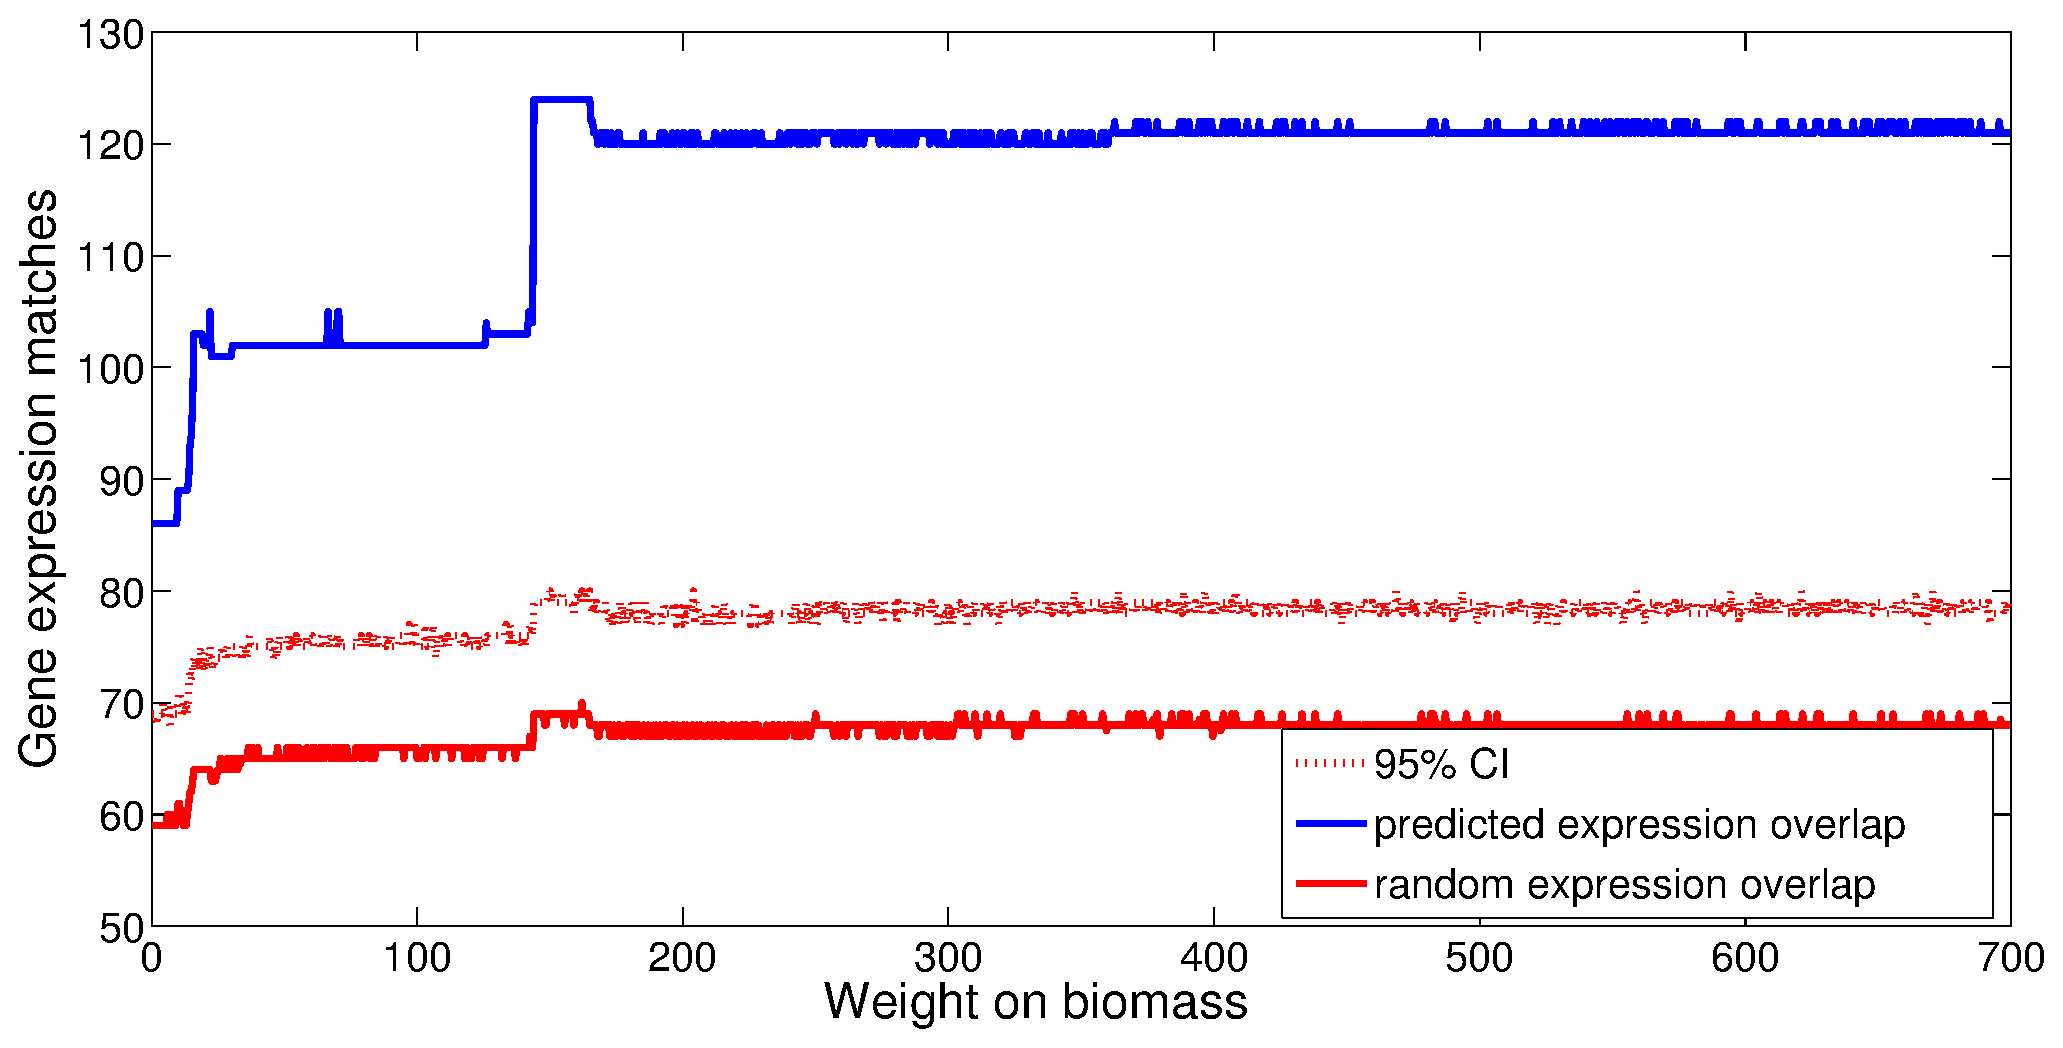
\includegraphics[width=\textwidth]{randGene_noFit}
  \caption{Linear MoMA} 
  \label{fig:randGene_noFit}
\end{subfigure}
\\
\begin{subfigure}[b]{\textwidth}
  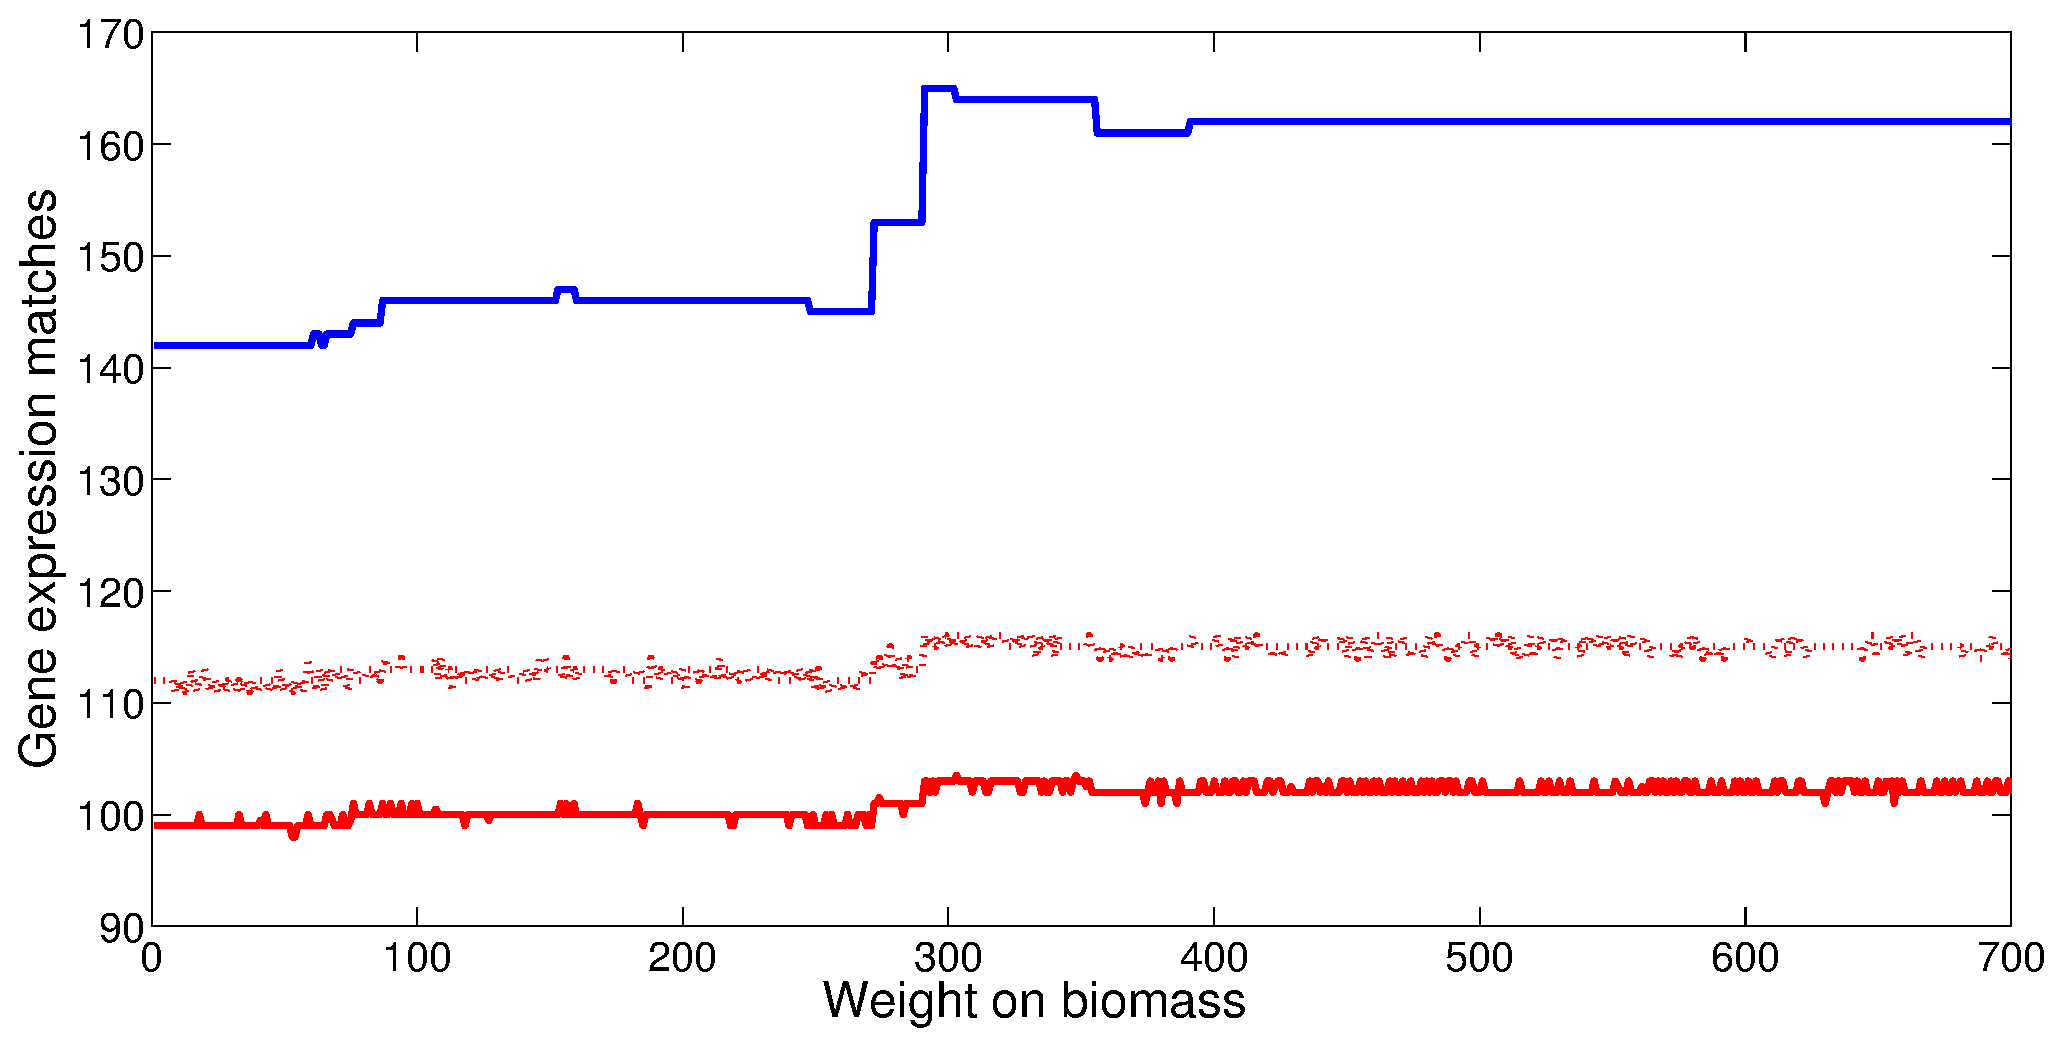
\includegraphics[width=\textwidth]{randGene_noFit_QP}
  \caption{Quadratic MoMA} 
  \label{fig:randGene_noFit_QP}
\end{subfigure}
\\
\end{tabular}
\caption{\hl{It is empty}} 
\label{fig:wMoMA_expMatch}
\end{figure}


Interestingly, the weight and corresponding fitness that agrees most
with the experimental predictions is sub-optimal in both the quadratic
and linear cases, suggesting that the s288c strain was not fully
adapted to the YPE environment when the expression was assayed.  To
compare directly with geometric FBA (a min-L1 norm solution), we found
that geometric FBA had 123 concurring genes whereas weighted linear
MoMA had 124; similarly, a min-L2 norm FBA solution in Ethanol had 162
agreeing solutions and weighted quadratic MoMA had 165, showing that
weighted MoMA can do at least as good as the gold standards for de
novo FBA solutions in predicting accurate fluxes.


\subsubsection{Simulated adaptation induces complexity in sub-optimal solutions}

Previous work by \hl{Nishikawa et al.} explored the complexity of optimal
and sub-optimal flux vectors, finding that generally the sub-optimal
solutions have more active fluxes than the optimal solutions. We found
a similar trend where, once growth is non-zero, the initial flux state
has more active reactions than in the ancestral environment (glucose;
red dashed line) or than in the more adapted stages in the current
(ethanol) environment.


\begin{figure}
\centering
  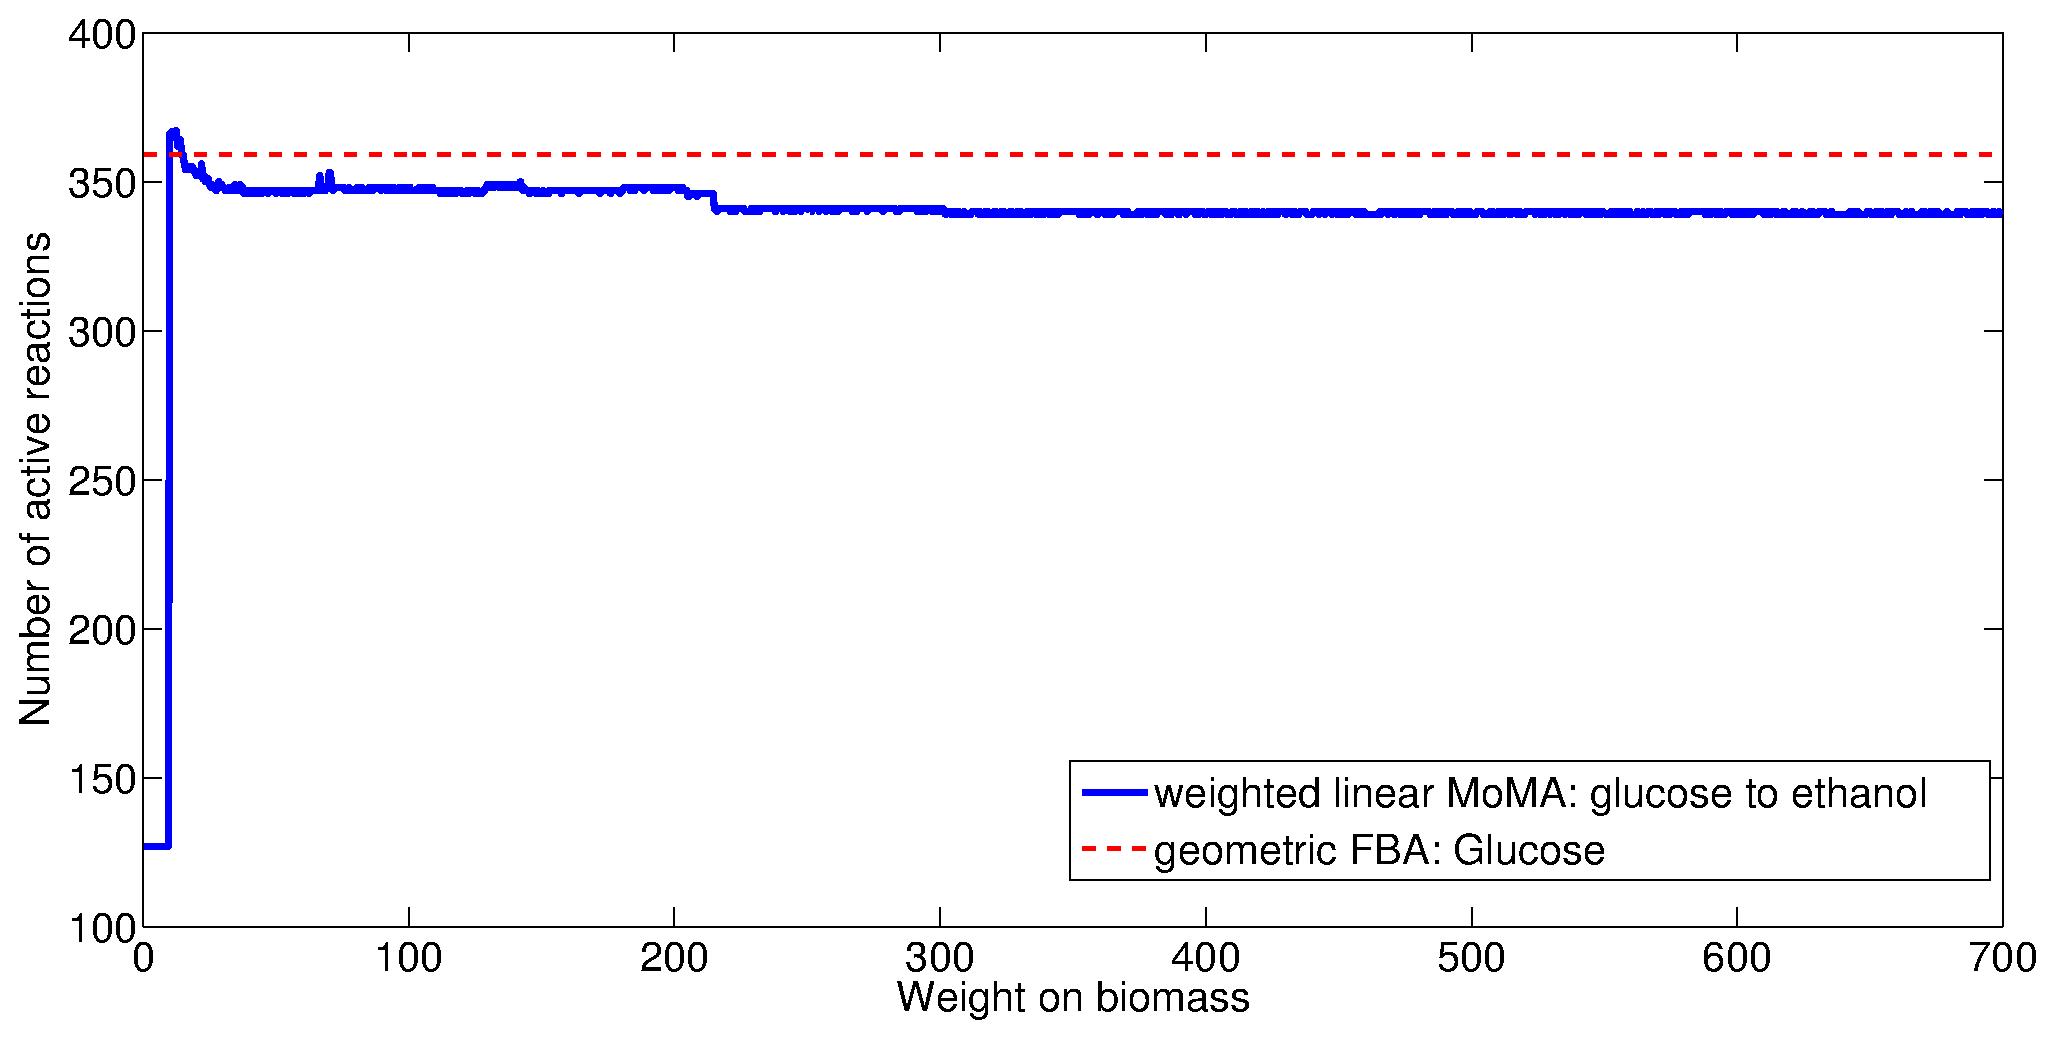
\includegraphics[width=\textwidth]{complexityEth}
  \caption{\hl{it is empty}} 
  \label{fig:complexityEth}
\end{figure}


\subsection{Adaptive mutations with objective weights}

Aside from the problem of separating the fitness function from the 
optimization objective function, there is the issue of combining traditional flux
restriction mutations, which are known as \emph{hard constraints}, which may
result in an unsolvable system --- an almost certainly undesirable
effect of this mutation modeling formalism. Instead, it would be
better if mutations could be modeled as \emph{soft
  constraints}. Concretely, whereas hard constraints are enacted in
the actual constraints of the optimization problem, soft constraints
merely change the objective. This means that multiple soft constaints
combined together under some mutational model would be compatible in
the sense that they wouldn't unexpectedly result in an unsolvable
system. FALCON provides two possible avenues for soft constraints:
expression level and expression variation. \emph{However, it is not
  clear yet what expression variation really means, so further
  investigation is necessary.}


Perturbations other than flux constraint are possible. One problem
with flux constraint occurs when we select two different reactions
that are to have their flux increased. It is all too easy for these
perturbations to be viable and even beneficial under weighted MoMA,
but for the corresponding double mutant to be inviable. This is true
for even small increases in flux, however one defines small, due to
the rigidity of flux constraint. For instance, if we only have a
specific amount of subtrate to work with, and a particular pathway is
already operating at optimal capacity, raising the lower bound to a
value greater than that capacity will result in zero fitness, which is
certainly not the intent of what we wish to capture nor is it
physically realistic. An alternative that can address this issue is to
perturb the linear objective vector. When performing growth
optimization in FBA, normally only the biomass pseudo-reaction has a
non-zero (positive) entry. Nonzero values for any other entry could
only decrease the flux. In weighted MoMA nonzero values could prove
potentially beneficial, as they may push the system in a direction
that is more in line with growth optimization and less in line with
MoMA.

An example for both the quadratic and linear cases exemplifies the
difference in smoothness obtained from using either a linear or
quadratic objective for weighted MoMA with objective weights (mutations)
on a particular reaction (\Fig~\ref{fig:wMoMA_smoothness}).


\subsection{Adaptive trajectories and evolutionary path analysis}

Phenotypes involving a small number of mutations have had their
adaptive paths analyzed systematically (\citep{Poelwijk2007,Weinreich2006, 
Khan2011, Chou2011}; four or five mutations). In \citet{Weinreich2006}, all
mutations occur on a single enzyme, and even in such a localized case,
sign epistasis, which gives rise to evolutionary traps, occurs for the
majority of mutational paths.

In a genome-scale metabolic model, we observe that while the majority
of paths are not likely to have a problem, once eight or nine genes are
involved, the average number of paths to reach the optimum without
experiencing a trap are only ~65\%. This demonstrates that the
presence of traps are heterogeneous, just as in the single-enzyme
experiment of \citet{Weinreich2006}, suggesting that the order of
mutations often matter to a very significant degree in evolution.

The fact that many unobstructed evolutionary paths are observed at the
genome-scale (\hl{cite figure}) suggests that evolution is, in
general, not very predictable. However, if we consider that neutral
mutations are unlikely to fix in a population, the number of viable
paths would greatly decrease (\suppOrApp
Section~\ref{sec:pathAnalysis}). Interestingly, in every experimental
case (Table~\ref{tab:threeAdaptEvoDats}), only a single fitness peak
appears to be present
\citep{Lunzer2005,Weinreich2006}. When we consider simulations from
genome-scale models instead of isolated pathways or single protein, we
still observe the single fitness optima for five mutation sets, but
once we consider eight mutations, every set of eight or more mutations
presents with multiple local optima. This suggests that evolution
becomes not only less predictable when we look at evolution of larger
systems or evolution at a large time scale, but also less likely to
reach the global optimal fitness.



\hl{include 2 subfigures}

\subsubsection{Software for evolutionary path analysis}

Storing all evolutionary paths in memory or disk can become 
intractable. For instance, even 10 mutations has $10! \approx
3.6$ million possible paths, but only $2^{10} = 1,024$ mutant
combinations. Due to this difficulty, we have created software to allow 
the dynamic exploration and analyses of these paths. 

The C programs for dynnamically performing analyses on text files
containing fitness data for all combinations of $n$ mutations can be
found online, and additional information and and examples related to
usage is available (\suppOrApp Section~\ref{sec:pathAnalysis}).

Notes: See Weinreich 2007 for really nice discussion and refs:
%http://webpub.brown.edu/Research/Weinreich/WeinreichPublications/Poelwijk_etal2007.pdf
%http://onlinelibrary.wiley.com/doi/10.1111/j.0014-3820.2005.tb01768.x/pdf

Note: also discuss the trends found for sign epistasis, if any, in the two recent science papers:
Khan et al.
Chou et al.

\subsubsection{Small beneficial mutants exhibit positive epistasis}

Prior studies using metabolic models have shown that deleterious
mutations tend to exhibit negative epistasis for stronger mutations
and positive epistasis for weaker mutations (\citep{He2010, Xu2012};
\hl{add full figure from MS1}). The reason for positive epistasis
being prevalent for deleterious mutations is that most of them occur
in essential pathways, and one mutation will buffer against the
effects of a second mutation (\citep{Xu2012}). Somewhat surprisingly,
we also see that predictions for epistasis involving weakly beneficial
mutations also tend to have positive epistasis (\hl{cite some
figures}). This trend is verified for two experiments involving
multiple genes (as in our simulation) where fitnesses are readily
calculated (\citep{Chou2011, Khan2011}; Table~\ref{tab:pairwiseBeneEpi}).

\begin{table}
\newcommand{\hlB}{\cellcolor{blue!20}}
\newcommand{\hlR}{\cellcolor{red!20}}
\centering
\begin{tabular}{cc}
\begin{subtable}[b]{0.5\textwidth}
\caption{\citet{Khan2011}}
\begin{tabular}{cccccc}
fitness &   & t           & s           & g           & r           \\
1.145   & t &             &             &             &             \\
1.108   & s & \hlB -0.060 &             &             &             \\
1.030   & g & \hlB -0.027 & \hlB -0.014 &             &             \\
1.015   & r & \hlB -0.056 & \hlB -0.004 & \hlR 0.005  &             \\
1.003   & p & \hlR  0.049 & \hlR  0.078 & \hlR 0.045  & \hlR 0.007  \\
\end{tabular}
\end{subtable}
&
\begin{subtable}[b]{0.5\textwidth}
\caption{\citet{Chou2011}}
\begin{tabular}{ccccc}
fitness &       & gshA        & GB          & fgh         \\
1.509   & gshA  &             &             &             \\
1.166   & GB    & \hlB -0.120 &             &             \\
1.142   & fgh   & \hlB -0.100 & \hlB -0.012 &             \\
1.096   & pntAB & \hlB -0.040 & \hlR  0.021 & \hlR 0.029  \\
\end{tabular}
\end{subtable}
\\
\end{tabular}
\caption{Pairwise epistasis values (calculated multiplicatively) from 
two experimental systems. \hl{Need to describe mutations and systems}.}
\label{tab:pairwiseBeneEpi}
\end{table}


The trend for increasing negative epistasis as mutations become
increasingly beneficial (also termed \textit{diminishing returns
epistasis}; \citep{Chou2011}) can be easily understood in most
contexts, including metabolism, due to the fact that in any given
environment there must be a physiological maximum value for most
phenotypes, including growth rate of a cell or individual organism.
Thus, if one mutant is extremely beneficial, it proportionally limits
the effect another beneficial mutant might have when combined
together.


This trend in epistasis can also be captured by our constraint-based
modeling framework. After screening \textit{in silico} for beneficial
mutations (Section~\ref{sec:epiBeneMethodSS}), we can examine trends in
pairwise epistasis as a function of the single mutant fitnesses 
\Fig~\ref{fig:beneEpiPairwise}. A fairly distinct border appears
to be present between the region that has some positive epistasis and
no positive epistasis. By considering that an epistatic cutoff (call
it $\epsilon_c$) is employed, we may use the multiplicative epistatic
relationship $W_{xy} - W_x W_y > \epsilon_c$, which yields the
reciprocal function $W_y > \frac{W_{xy} - \epsilon_c}{W_x}$ for fixed
$W_{xy}$, which limits the region in which positive epistasis, as
defined by $\epsilon_c$, can occur. Since $W_{xy}$ is not a constant,
there may be some variation in the actual trend from a true reciprocal
function. The reason the mean has a similar curve is because of the
decreasing marginal benefits of epistasis, which means correspondingly
greater magnitudes for negative epistasis as the single mutant
fitnesses increase.

%Change to two col later?
\begin{figure}
\centering
\begin{tabular}{c}
\begin{subfigure}[b]{\textwidth}
  \includegraphics[width=\textwidth]{beneEpiMean_tmp}
  \caption{mean epistasis} 
  \label{fig:beneEpiPairwise:mean}
\end{subfigure}
\\
\begin{subfigure}[b]{\textwidth}
  \includegraphics[width=\textwidth]{beneEpiPerc_tmp}
  \caption{percent of positive epistasis}
  \label{fig:beneEpiPairwise:perc}
\end{subfigure}
\\
\end{tabular}
\caption{The mean epistasis (\ref{fig:beneEpiPairwise:mean}) and percentage
  (\ref{fig:beneEpiPairwise:perc}) of positive epistasis for epistases such
  that $\left|\epsilon\right| \ge 0.01$.}
\label{fig:beneEpiPairwise}
\end{figure}

The distribution of epistases arising from beneficial mutations is
highly similar to that found in natural biological systems that are
also described by population genetic models
(\Fig~\ref{fig:epiBeneDist}; \citep{Martin2007a}). Interestingly, the
small-scale data from \citet{Martin2007a} is from an RNA virus (VSV),
whereas our stoichiometric models are not designed for modeling
viruses. Nonetheless, the trend remains similar, suggesting that this
is a trend that extends across completely different types of models as
well as from the fitness of complex life forms and simple non-living
viruses. This excellent fit requires that an appropriate distribution
of fitnesses is sampled according to extreme value theory (EVA;
Section~\ref{sec:epiBeneMethodSS}; \citep{Orr2005, Orr2003}).


\begin{figure}
\centering
  \includegraphics[width=\textwidth]{99p9_epi_YPD_tmp}
  \caption{Distribution of epistases arising in a yeast model from
beneficial mutations sampled according to EVA.}
  \label{fig:epiBeneDist}
\end{figure}

\section{Discussion}

We have developed a data-driven modeling framework in the
constraint-based metabolic modeling family that allows the exploration
of combinatorial epistases and reproduces trends seen from studies in
the forefront of evolutionary research \citep{Martin2007a, Chou2011,
Khan2011}. Contemporaneous, theoretical insights in to how a general
clas of mechanistic models, encompassing those used in this study,
give rise to traditional population genetic models such as Fisher's
geometric model \citep{Martin2014}.  The methodologies described in
this paper should have applications in diverse fields due to their
reliance on mechanistic models available for many organisms
\citep{Monk}.

The questions are often
difficult or impossible to assess experimentally due to limited
resources.  In genome-scale models, to our knowledge, only microbial
epistasis has so far been studied for all enzymes (often referred to
as genome-scale in this context). This is due to several factors.

One issue is that these computations can still take a significant
amount of time, and the increase in model size of Human Recon 2 over
Yeast can cause even a relatively simple FBA run to go up by an order
of magnitude.  This problem is compounded by the increase in the
number of genes in the human model, since computing epistasis consumes
space and time as $O(n^2)$ where $n$ is the number of genes in the
model. More important than this issue, which might be overcome with
enough computational resources, is the issue of an objective
function. It has been shown numerous times that FBA with a biomass
objective can be a reasonable approximation to what a microbe is
trying to achieve metabolically
\citep{Schuetz2012, Fong2004, Varma1994}. While Recon 2
is equipped with a ``generalized biomass reaction'', it is not clear
what the meaning of this is, and it certainly seems unlikely to
estimate the metabolism even of fast-growing cancer cells \hl{(cite
  Locasale?)}. We propose FALCON as a method to get around this issue
for non-microbial models.

Another advantage of FALCON is that it allows one to directly probe
mutations that are represented as gene expresion perturbations. A
decreased level of gene expression may also be metabolically
equivalent to the effect of a missense mutation, for example. This
allows a different sampling strategy than before; for instance, we
could observe how uniform expression restriction compares to uniform
flux restriction~\citep{Xu2012}. Assuming an accurate model of
enzyme-complex expression measurement, the former should be the more
realistic model.

A limitation is that we have only considered metabolic genes and their
effect on steady-state metabolism. While in principle a similar method
could be applied to whole cell models \hl{cite myco and e.coli}, the
computation time would not be feasible to the screening for beneficial
muatations, nor of exploring them combinatorally, as the time needed
for a single mutant takes at least a day even in the smallest
bacterial model \hl{cite}. Future isnights into improving the
efficiency of whole cell models, or making a compromise on which
systems are simulated (e.g. rFBA, \citep{Covert2001}), may improve
these efforts.

\section{Methods}
\label{sec:epiBeneMethod}

\subsection{Mutation screening and sampling}
\label{sec:epiBeneMethodSS}
\hl{it is empty}

\section{TODO}

\hl{need more background}


\hl{include weighted moma subsection to introduce need for FBA
in conjunction with FALCON; tie in this multiobjective function
to the multiobjective optimality found by Shuetz}

\hl{add images of Lin's experimental data}

\hl{actually try to use FALCON for GxG interactions, discuss caveat
that it is possible that influencing one enzymatic gene's abundance
could affect another enzymatic gene's abundance, and we can't directly
take this into account in our model}

\hl{discuss C software I developed for analysing adaptive trajectories;
need to update to work with FALCON}


\hl{briefly discuss FBA weight possibility}


\hl{Since beneficial mutations are relatively rare, and since
combining multiple mutants in the lab is increasingly difficult for
the more mutations that are to be combined, an \textit{in silico}
analysis can shed light on what may be expected in adaptive
evolution.}

